\documentclass[letterpaper,twocolumn,10pt]{article}
\usepackage{iftex}
\ifXeTeX
  \makeatletter
  \@namedef{ver@breakurl.sty}{2026/10/30 Native XeTeX URL handling}
  \makeatother
\fi
\usepackage{hyperref}
\usepackage{usenix}
\usepackage{xurl}
\ifXeTeX
  \microtypesetup{spacing=false,kerning=false}
\fi
\usepackage{amsmath,amssymb,booktabs,tabularx,graphicx}
% Generated from raw benchmark JSON; do not edit.
\newcommand{\BenchTrials}{20}
\newcommand{\SecurityCases}{32}
\newcommand{\SecurityObservations}{640}
\newcommand{\UnauthorizedEffects}{0}
\newcommand{\TypedDisagreements}{0}
\newcommand{\SignatureFalseAccepts}{520}
\newcommand{\GateMedian}{0.498}
\newcommand{\GatePninetyfive}{1.688}
\newcommand{\ChannelObservations}{240}
\newcommand{\CleanSuccesses}{20}
\newcommand{\PatternCollisions}{6}
\newcommand{\CollisionTrials}{1000}

\title{OpenATT: Scoped Controller Evidence Without Promoting Contact to Consent}
\author{Research draft\\Authorship to be finalized}
\date{October 31, 2026}
\begin{document}
\raggedbottom
\maketitle
\begin{abstract}
Tactile observations do not automatically identify a consenting person or authorize an agent action. We present OpenATT, a local Python reference for bounded force/time acquisition, challenge-dependent contact-pattern appraisal, signed controller reports and separate exact-action permission. A shared verifier atomically consumes evidence context and grants with a local receipt. Generated-trace benchmarks expose sensitivity to noise and timing, and an explicit short-code experiment records old traces matching new patterns. Finite policy cases and concurrent duplicate schedules exercise the enforcement boundary; an equally expressive typed control matches serial outcomes. No hardware sensing, user authentication, physical actuation, general composition theorem or novel cryptography is claimed. The artifact makes those distinctions executable and identifies the capture assumptions a real fixture must justify.
\end{abstract}
\section{Introduction}
An agent operating through a human-facing fixture can observe a button press,
contact event or haptic response. These observations are useful, but the inference
from ``contact happened'' to ``the authorized customer agreed'' is unjustified.
A controller can report a force pattern without identifying the toucher or
establishing willingness. A signed packet does not repair an untrusted sensor
path or make an old raw trace a fresh physical interaction.

OpenATT (Open Agent Tactile Trust) implements scoped controller evidence and
keeps it separate from permission. A stored challenge defines a short/long
contact pattern. A configured controller signs a bounded force/time trace and
the exact challenge. The verifier reprocesses the signal and checks binding,
current owner permission and required guarantees before creating one durable
local receipt. Contact reports never supply human consent or proximity.

This report provides concrete CSV acquisition, integer-unit signal processing,
controller signing, a shared transaction gate, attack cases and generated-trace
benchmarks. It does not report hardware sensing, human authentication, haptic
actuation or physical deployment. That distinction matters because the strongest
assumption is the trustworthy sensor-to-signing path, which the software profile
cannot create on its own.

\paragraph{Supported contribution.}
The artifact makes contact/consent separation and short-pattern limitations
executable. It supplies negative results: increased noise and timing variation
reduce acceptance, and an eight-bit pattern admits collisions across different
challenges. Signatures, hysteresis and database transactions are established
techniques. The equally expressive typed control matches the observed serial
policy behavior; no stronger authorization property or formal proof is claimed.
Research on sound composition and efficient evidence acquisition remains ahead.


\section{Problem and Threat Model}
\subsection{A reporting controller, not a human identity}
The example action records fixture contact in a local ledger. A controller owns
an Ed25519 key and can access a force/time acquisition process. The owner signer
separately delegates this exact recording action. The action is deliberately not
a door unlock or package release: those require independent actuator enforcement
and may require a stronger human authorization ceremony.

The report authenticates a configured controller's assertion about its trace.
Physical association, correct calibration, trustworthy analog sensing and capture
after the challenge are assumptions of the acquisition process. The SDK accepts
bounded samples; signing an arbitrary existing CSV file does not prove that those
samples were newly collected. We expose this limitation rather than equating
fresh signature response with fresh physical contact.
\subsection{Exact actions and separate permission}
An action is an immutable snapshot of principal, operation, resource, purpose and
all tool arguments. Let $h(a)$ be its SHA-256 digest under the bounded local JSON
profile. A stored challenge includes $h(a)$, business audience, modality, a random
128-bit nonce, a random 128-bit session identifier, issue time and expiration.
The default lifetime is 30 seconds and the maximum is 120 seconds. The signed
response must match the complete server-stored challenge, not just a caller's
claim that a nonce was once issued.

A different configured owner key signs a one-use grant containing the principal,
audience, $h(a)$, allowed modalities and a bounded validity interval. An attester
key cannot substitute for that grant. Registration stores the token digest;
re-registration never resets revocation or consumed state. These are demo
administrative roles: the implementation does not establish legal identity,
verified account enrollment, a human consent ceremony or a hardware root of trust.

\subsection{Adversary and assumptions}
An attacker may alter untrusted observations, replay evidence, obtain a legitimate
key of its own, substitute any action field, relay a live exchange and schedule
concurrent requests or revocation. The verifier code, configured key maps,
owner signer, gateway clock and local database administrator are trusted.
The configured attester is trusted to report within its documented capture
assumptions. A compromised attester may sign a false observation for a fresh
challenge. We include this limitation rather than treating signature validity as
sensor truth.

The language model, if a future integration includes one, does not select its own
trusted keys, change the action contract, create an owner signature or bypass the
gate. The released benchmark contains no language model. It measures structured
protocol behavior, not resistance to arbitrary prompt injection or leaks through
other tools and outputs.


\section{Alternatives and Research Position}
Touch and haptic authentication have a substantial history. TouchIn combines
knowledge of a gesture with behavioral and physiological features~\cite{touchin}.
Recent tele-robotic work uses force-feedback dynamics for user
identification~\cite{haptic}. OpenATT is neither a biometric classifier nor a
competitor to their user-identification accuracy; it has no participant dataset.
Its pattern is public and contains only eight bits, so it is not an identity
secret.

WebAuthn separately specifies user-presence and user-verification checks and
relying-party validation~\cite{webauthn}. An arbitrary force threshold or
controller signature does not instantiate that ceremony. A trusted authorization
flow can supply permission; a tactile event can supply a distinct reported
observation. Combining them must preserve their meanings.

RATS separates evidence from appraisal~\cite{rats}. Analog sensor-injection
research such as WALNUT demonstrates that digital processing can begin with
adversarial physical inputs~\cite{walnut}; a signature downstream cannot establish
the integrity of that upstream physical measurement. CaMeL and Fides enforce
control/data-flow policies around agents~\cite{camel,fides}. OpenATT uses a
trusted action gate but does not implement their planners, prove their properties
or reproduce their agent evaluation.

Accordingly, signed controller reports and exact grants are engineering
foundations. The prospective scientific question is whether a common evidence
contract can preserve non-equivalent guarantees across changing perceptual
contexts and acquire adequate support at lower cost. The current work supplies
an inspectable tactile boundary and limitations, not that general result.


\section{Design and Implementation}
\subsection{Bounded trace and contact segmentation}
Samples are pairs of integer milliseconds and millinewtons. The profile accepts
10--512 samples over at most five seconds. Acquisition begins at relative time
zero; timestamps must strictly increase with gaps no larger than 20 ms. Force
must lie between zero and 20,000 mN. CSV has exactly the header
\texttt{time\_ms,force\_mn}; files are bounded to 64 KiB. CSV alone has no
cryptographic authenticity.

A hysteretic segmenter begins contact at 500 mN and ends it at 200 mN. Contacts
shorter than 40 ms, traces ending during contact, malformed timestamps and
acquisition gaps are rejected. These are explicit fixture settings, not
calibrated physiological or hardware thresholds. The verifier repeats the
segmenter rather than trusting controller-supplied contact labels.

\subsection{Public short/long challenge pattern}
SHA-256 of the complete challenge supplies eight pattern bits. Each bit selects
a 100 or 200 ms contact; intended gaps are 100 ms. Verification allows duration
error of at most 20 ms and gaps of 80--120 ms, including the initial gap. The
profile requires exactly eight contacts. The response signs the complete
challenge, resource name, profile and raw bounded samples.

The pattern has just $2^8=256$ possible values. It is an acquisition-consistency
check, not a secret, distance bound or cryptographic nonce. An old trace may match
a new code. A compromised controller can generate a matching trace directly.
The full signed 128-bit nonce/session prevents transplanting an old signed
response, under the configured-key assumption, but does not prove new physical
capture if the controller signs stale samples. This is why the reported-contact
guarantee retains its explicit trusted sensor-path assumption.

The simulator emits 10 ms samples at nominal 1,000 mN contact force, with bounded
uniform force noise and contact-duration jitter. These functions generate test
fixtures; the package does not label them sensor recordings or assume a real
controller follows them. A real acquisition adapter must maintain the documented
capture ordering and protect the sensor-to-signing path.
\subsection{Acceptance and transaction boundary}
For evidence $e$, grant $g$ and action $a$, the intended rule is
\begin{align}
\mathsf{Receipt}(a) \Rightarrow {}& \mathsf{SignatureValid}(e) \nonumber\\
 &\land\ \mathsf{ChallengeStoredAndUnused}(e,h(a)) \nonumber\\
 &\land\ \mathsf{ScopeAndTimeValid}(g,a) \nonumber\\
 &\land\ \mathsf{Supported}(e,\mathsf{Contract}(a)) \nonumber\\
 &\land\ \mathsf{CurrentAndUnused}(g).
\end{align}
This is a design invariant supported by finite tests, not a mechanized proof.
The gateway derives supported guarantees from its own validators. A signed
adapter field such as \texttt{trusted=true} is rejected as an unknown field.
Unsupported requirements such as physical proximity or human consent cannot be
supplied by relabeling a valid signature.

Cryptographic and modality appraisal precede a SQLite \texttt{BEGIN IMMEDIATE}
transaction. After acquiring the write lock, the gateway rechecks time, issuer
revocation, complete stored challenge and grant state. Receipt insertion and
challenge/grant consumption then commit together. An insertion failure rolls
back consumption; restarts retain replay state. Revocation committed before this
boundary prevents a later receipt. Revocation after an already committed receipt
cannot undo history.

The sole effect is an append to this local receipt ledger. There is no callback
that silently sends a remote command inside this claim. A payment, actuator,
message, downstream database or later physical event needs its own participating
commit semantics. The usual database transaction is an implementation foundation,
not a novel consistency mechanism.

\subsection{Bounded parsing and role separation}
The shared package signs a versioned kind/issuer/body envelope using
domain-separated Ed25519~\cite{eddsa}. The local JSON profile permits bounded
integers, strings, arrays, objects, booleans and null, with sorted ASCII-escaped
keys and fixed separators. It rejects duplicate keys, floats, nonfinite values,
excessive nesting, large messages, unknown fields and boolean timestamps. The
maximum encoded message is 32 KiB. These choices reduce parser ambiguity; they
are not JOSE, COSE, RFC 8785 or compatibility with the umbrella's draft schema.
Evidence trust maps are scoped by modality; a display key cannot act as a
controller without explicit configuration. The private keys never appear in released reports. Evidence is signed, not
encrypted; public claims and tactile traces must not contain secrets.


\section{Evaluation}
\subsection{Generated-signal reliability}
The signal suite pairs twelve conditions within each of \BenchTrials{} explicit
scenario seeds: uniform force-noise bounds of 0, 100, 300 and 600 mN crossed with
uniform contact-duration jitter bounds of 0, 10 and 30 ms. It performs
\ChannelObservations{} generated trace trials. Success means that an honest
controller's \texttt{respond} routine accepts the trace, recomputes the pattern
and emits a signed response. Failure reasons and processing costs are retained.
No physical sensor, person or actuator participates.

\begin{figure*}[t]
\centering
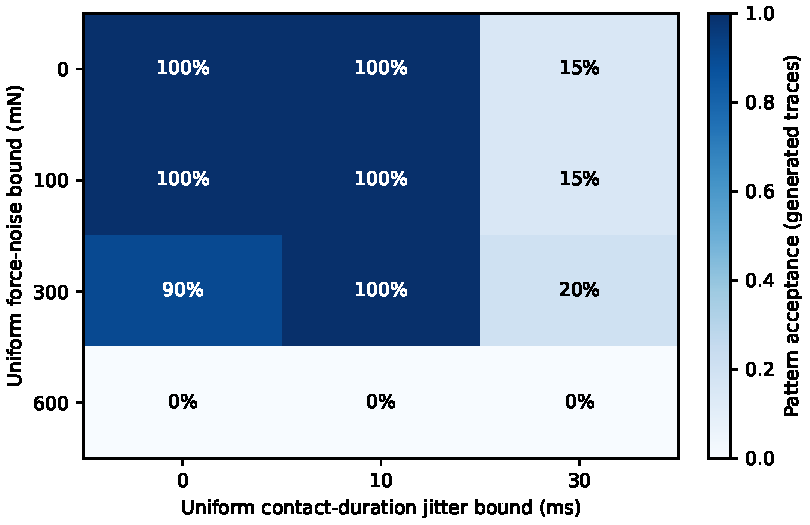
\includegraphics[width=0.75\textwidth]{artifacts/channel.pdf}
\caption{Pattern acceptance on generated force/time traces. Each cell contains
20 scenario seeds; conditions share seeds. The data describe fixture-profile
sensitivity, not a human-authentication rate or sensor accuracy.}
\label{fig:signal}
\end{figure*}

The zero-noise, zero-jitter condition accepted
\CleanSuccesses{}/\BenchTrials{} traces. Large timing variation reduced acceptance;
600 mN noise produced no accepted traces in the recorded conditions. Not every
intermediate condition is monotonic because noise changes crossing times in a
thresholded signal. The fixed finite scenario family does not support a general
noise-tolerance threshold. Rejected-trace processing is often faster than valid
signing, so pooled timing must not be interpreted as a throughput advantage.
Processing time excludes the simulated multi-second interaction duration.

\subsection{Short-pattern collision experiment}
We preserve one generated old trace and test it against \CollisionTrials{}
different challenge contexts. Its segment pattern matched
\PatternCollisions{} contexts. This is compatible with a small 256-code space,
not a cryptographic break. An old signed envelope still contains its original
nonce/session and fails full binding in a new stored interaction. Conversely, a
controller that signs old raw samples for a colliding new pattern can pass the
software checks. Capture freshness is an acquisition assumption, not a property
established by the eight tactile bits. The benchmark records this negative
result explicitly.
\subsection{Policy controls and schedules}
The serial suite repeats every named case \BenchTrials{} times with fresh keys,
challenges and temporary SQLite state. It includes changed principals, actions,
resources, purposes and arguments; altered signatures; unconfigured keys; session
and nonce transplantation; wrong audience; expired challenges and grants; grant
and issuer revocation; unregistered permission; wrong grant scope/modality;
consumed replay; malformed observation profiles; unsupported guarantees and
unaccepted assumptions. Modality-specific cases extend this common taxonomy.

An intentionally weak signature-only ablation ignores scope, freshness and
permission. It isolates why authentication alone is insufficient; its failures
are not evidence against correctly configured existing authorization. An equally
expressive sequential typed-policy control separately checks the same expected
challenge, action, supported guarantees and permission state. It shares
cryptographic and modality validators with the gateway and is not an independent
audit, full IFC implementation or reimplementation of published agent defenses.

The concurrency suite runs \BenchTrials{} trials of eight duplicate attempts
released together; each must produce exactly one receipt. Another
\BenchTrials{} trials hold the write boundary, revoke the grant and then release a
worker's commit. Every such prior-revocation schedule must produce zero receipts.
This is a deliberately selected serialized order, not an exhaustive scheduler
exploration. Tests also check rollback, expiry at the boundary and replay after
restart.

\subsection{Interpretation}
Across \SecurityObservations{} serial case observations
(\SecurityCases{} cases per trial), the gateway produced
\UnauthorizedEffects{} unauthorized new local receipts and
\TypedDisagreements{} disagreements with the typed control. The weak
signature-only check accepted \SignatureFalseAccepts{} observations that violated
the specified policy. Mixed accepted/denied gate processing had median
\GateMedian{} ms and nearest-rank p95 \GatePninetyfive{} ms. These one-host
measurements include SQLite work for accepted requests, but are not a matched
latency comparison with the control or an end-to-end physical delay.

Two limitation cases deliberately accept valid structured responses: transparent
live forwarding when no proximity guarantee is required, and a configured
attester producing a plausible report when sensor truth is not required. These
are modeled traces, not physical relay or compromised-device experiments. Requiring
proximity or consent is separately denied. Denial is not a result demonstrating
those properties. Channel trials and policy cases are distinct suites; the
runnable demos combine channel parsing, signature appraisal and effect insertion.

\subsection{Validity and missing measurements}
Signal seeds are deterministic, key material and security challenges are fresh,
and all processing measurements come from one host. The force model, thresholds
and attack schedules were selected by the implementation authors. Per-condition
Wilson intervals are descriptive; paired conditions are not independent trials
that can be pooled into a deployment security rate. We have not measured real
force calibration, skin/material variation, user behavior, motor control,
controller compromise, haptic relay, classifier discrimination or secure hardware.
Future studies require those measurements and independent review before claiming
physical reliability or human authorization.


\section{Discussion and Next Steps}
\paragraph{Contact evidence has a small meaning.}
A valid report means that a configured controller signed samples satisfying a
known fixture profile for this interaction, under its sensor-path assumptions.
It cannot tell whether a person, robot, prerecorded trace or malicious firmware
produced them. No amount of relabeling makes this equivalent to consent. A
contract requiring an unsupported guarantee must deny the action, even when
every reported contact matches.

\paragraph{Stronger primitives are complementary.}
Protected sensor firmware, attestation, authenticated acquisition, calibrated
hardware and a user-approved transaction can justify additional claims. Those
claims need their own evidence and failure analysis. They should not be inferred
from a longer contact pattern alone. A deployment may not need tactile evidence
at all when a trusted API and appropriate consent flow already authorize the
exact action.

\paragraph{What remains research.}
The shared core checks one modality per receipt. It is not yet a composition
calculus, dependency invalidation engine or selective acquisition planner. OpenAVT
remains an independent voice implementation. OpenAST's fresh display response and
OpenATT's contact report cannot be substituted merely because both are signed.
Future handoffs must preserve resource, purpose, episode, assumptions and
supporting dependencies. A useful scientific result would establish that rule
or reduce acquisition/intervention cost without weakening the strongest policy
control. The present implementation demonstrates neither advantage.

The practical next step is a bounded hardware fixture with authenticated capture
ordering, protected signing keys and a cooperating backend. Human studies and
hazardous actuation are unnecessary for the current negative-result reference;
any later consent or usability claims need an appropriate study design.


\bibliographystyle{plainurl}
\bibliography{references}
\appendix
\section{Open Science and Reproduction}
Artifacts include source packages, SDK examples, CLI demos, tests, raw benchmark
JSON, per-case timings, dependency versions and measured source hashes. Report
generators derive manuscript numbers from the JSON; the evidence checker verifies
arithmetic and source hashes. Public synthetic fixtures are separate from trials.

Using Python 3.11 or later, install the local core and modality package, then run
the demo, tests, 20-trial benchmark, report generator and paper Makefile. READMEs
provide exact commands and dependencies. Fresh keys change byte hashes and timing;
scenario seeds and transformations are explicit. No PyPI publication is asserted.

\section{Ethics and Deployment Limits}
Fixtures are generated, without people, customer records or private keys. The
sole effect is a local receipt. No hardware, LLM, cloud deployment or independent
security review was evaluated. Deployment needs authenticated enrollment,
protected keys and justified capture/effect semantics. This research draft is not
a submitted paper, new cryptographic primitive or formal security proof.

\end{document}
